% =====================================================================
% Guía del estudiante -- Geometría 4° -- Trimestre I
% Hilo conductor: La vuelta al mundo en 80 días (Julio Verne), contada con nuestras palabras
% Temas (propuesta del trimestre I en curriculo/plan-anual.md, clases 003-011):
%   lineas, poligonos, cuadrilateros, tangram
% Plan y ejercicios: guia-periodo-I-lineas-y-poligonos.plan.md
% =====================================================================
% Plan del trimestre aprobado por la docente el 2026-09-18. Esta guía es todavía el borrador de
% la generación rápida del 2026-09-14: falta rehacerla con el proceso de tres etapas.
\documentclass[11pt]{article}
\makeatletter\def\input@path{{../../../../plantillas/estilo/}}\makeatother
\usepackage{mmcantillo}

% ======================== DATOS DE LA GUÍA ============================
\tipodocumento{Guía del estudiante}
\asignatura{Geometría}
\titulo{Líneas y polígonos alrededor del mundo}
\grado{4°}
\periodo{I}
\hiloconductor{La vuelta al mundo en 80 días}
% ======================================================================
% DBA: matematicas grado 4 · DBA 6 — Identifica, describe y representa figuras
% bidimensionales y tridimensionales, y establece relaciones entre ellas.
% (dba/matematicas/grados/grado04.tex). Paralelas y perpendiculares: DBA 7 de grado 2, como base.

\tikzset{etq/.style={font=\small\bfseries, text height=1.6ex, text depth=0.3ex}}

\begin{document}

\encabezado

% ---------------------------------------------------------------------
% 1. Frase introductoria
% ---------------------------------------------------------------------
% verificado: https://fr.wikisource.org/wiki/Le_Tour_du_monde_en_quatre-vingts_jours/Chapitre_3 — cap. III: «L'imprévu n'existe pas», responde Phileas Fogg (trad. propia)
\frase{Lo imprevisto no existe.}
{Phileas Fogg, en Julio Verne, \emph{La vuelta al mundo en 80 días} (1872), trad. propia}

% ---------------------------------------------------------------------
% 2. Introducción
% ---------------------------------------------------------------------
\seccion{Introducción}

Phileas Fogg, el protagonista de una novela de Julio Verne~\cite{verne}, lo
planeaba todo: a qué hora salía el tren, cuántos días duraba cada barco,
por dónde pasaba cada ruta. Por eso decía que «lo imprevisto no existe». La
geometría se parece a Fogg: con una regla, una escuadra y unas pocas
definiciones claras, podemos trazar y reconocer figuras sin dejar nada al
azar.

En este trimestre acompañaremos a Fogg y a su ayudante Passepartout en su
vuelta al mundo. En cada etapa del viaje encontraremos algo nuevo: las
líneas de los rieles del tren, los polígonos del barco, los cuadriláteros de
las calles y un rompecabezas de siete piezas.

\textbf{Al terminar este trimestre podrás:}
\begin{itemize}
  \item reconocer y trazar rectas paralelas, perpendiculares y secantes;
  \item identificar polígonos y nombrarlos según su número de lados;
  \item clasificar cuadriláteros por sus lados y sus ángulos;
  \item armar, desarmar y crear figuras con polígonos.
\end{itemize}

Este trimestre trabaja un Derecho Básico de Aprendizaje del Ministerio de
Educación Nacional~\cite{mendba}:

\begin{dba}[Grado 4 · DBA 6]
Identifica, describe y representa figuras bidimensionales y
tridimensionales, y establece relaciones entre ellas.
\end{dba}

En este trimestre trabajamos las figuras bidimensionales (planas); los
cuerpos tridimensionales llegarán en el tercer trimestre.

% ---------------------------------------------------------------------
% 3. Marco teórico
% ---------------------------------------------------------------------
\Needspace{8\baselineskip}
\seccion{Marco teórico: ¿Sabías que\ldots?}

\subsubsection*{Una novela por entregas}
Julio Verne publicó \emph{La vuelta al mundo en 80 días} por capítulos en un
periódico francés, entre noviembre y diciembre de 1872; el libro completo
salió en enero de 1873~\cite{cijv}. En la novela, Phileas Fogg apuesta
veinte mil libras a que puede dar la vuelta al mundo en 80 días.

\subsubsection*{Un viaje de 8 tramos}
El plan de Fogg tenía ocho tramos: de Londres a Suez (7 días), de Suez a
Bombay (13), de Bombay a Calcuta (3), de Calcuta a Hong Kong (13), de Hong
Kong a Yokohama (6), de Yokohama a San Francisco (22), de San Francisco a
Nueva York (7) y de Nueva York a Londres (9). Suma los días: ¡80
exactos!~\cite{verne}

\subsubsection*{Una periodista que lo hizo de verdad}
En 1889, la periodista estadounidense \textbf{Nellie Bly} leyó la novela y
decidió intentarlo. Dio la vuelta al mundo en solo 72 días, y un periódico de
Nueva York contó su viaje día por día~\cite{nwhm}.

\subsubsection*{Paralelas desde hace más de 2\,000 años}
El griego \textbf{Euclides} escribió en su libro \emph{Elementos} que las
rectas paralelas son las que están en el mismo plano y, aunque se alarguen
todo lo que se quiera hacia los dos lados, nunca se encuentran~\cite{euclides}.
¡Es la misma idea que usamos hoy!

\subsubsection*{Siete piezas ingeniosas}
El \textbf{tangram} es un rompecabezas que se inventó en China hacia el año
1800. Su nombre chino quiere decir «siete piezas ingeniosas». En 1817 llegó a
Europa y se volvió una moda: fue la primera gran fiebre de los
rompecabezas~\cite{britz}.

% ---------------------------------------------------------------------
% 4. Temas
% ---------------------------------------------------------------------
\tema{Líneas}\label{tema:lineas}

\begin{hilo}
En un club de Londres, Phileas Fogg apuesta con sus amigos que dará la
vuelta al mundo en 80 días. Esa misma noche sale en tren con Passepartout.
Mirando por la ventana, Passepartout nota algo: los dos rieles de la vía van
siempre juntos, a la misma distancia, y nunca se encuentran.
\end{hilo}

\Needspace{9\baselineskip}
Una \textbf{recta} es una línea derecha que no tiene principio ni fin: se
alarga sin parar hacia los dos lados. Si le ponemos un principio y un fin,
tenemos un \textbf{segmento}; si solo le ponemos un principio, tenemos una
\textbf{semirrecta}, como un rayo de luz que sale de una linterna.

\begin{center}
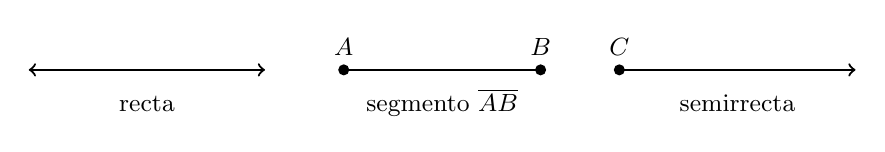
\begin{tikzpicture}[thick, every node/.append style={text height=1.6ex, text depth=0.3ex, font=\small}]
  \draw[<->] (0,0) -- (3,0);                   \node[below] at (1.5,-0.15) {recta};
  \draw (4,0) -- (6.5,0); \fill (4,0) circle (2pt) node[above] {$A$};
  \fill (6.5,0) circle (2pt) node[above] {$B$}; \node[below] at (5.25,-0.15) {segmento $\overline{AB}$};
  \draw[->] (7.5,0) -- (10.5,0); \fill (7.5,0) circle (2pt) node[above] {$C$};
                                               \node[below] at (9,-0.15) {semirrecta};
\end{tikzpicture}
\end{center}

\Needspace{7\baselineskip}
Dos rectas pueden estar en tres posiciones:

\begin{center}
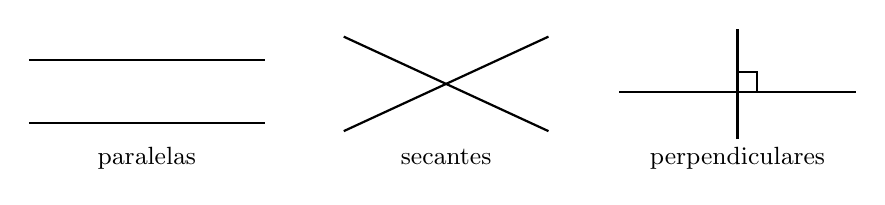
\begin{tikzpicture}[thick, every node/.append style={text height=1.6ex, text depth=0.3ex, font=\small}]
  \draw (0,0) -- (3,0); \draw (0,0.8) -- (3,0.8);  \node[below] at (1.5,-0.15) {paralelas};
  \draw (4,-0.1) -- (6.6,1.1); \draw (4,1.1) -- (6.6,-0.1); \node[below] at (5.3,-0.15) {secantes};
  \draw (7.5,0.4) -- (10.5,0.4); \draw (9,-0.2) -- (9,1.2);
  \draw (9,0.4) rectangle (9.25,0.65);          \node[below] at (9,-0.15) {perpendiculares};
\end{tikzpicture}
\end{center}

\begin{itemize}
  \item \textbf{Paralelas}: nunca se cortan, aunque las alarguemos. Se escribe $r \parallel s$.
  \item \textbf{Secantes}: se cortan en un punto.
  \item \textbf{Perpendiculares}: son secantes que forman cuatro
        \textbf{ángulos rectos}, como la esquina de una hoja. Se escribe $r \perp s$.
\end{itemize}

\begin{ejemplo}[Trazar con regla y escuadra]
Para trazar una \textbf{perpendicular} a una recta $r$ que pase por un punto
$P$: apoya un lado de la esquina recta de la escuadra sobre $r$ y deslízala
hasta que el otro lado pase por $P$; traza la línea.

Para trazar una \textbf{paralela} a $r$ por $P$: pon la regla sobre $r$,
apoya la escuadra en la regla y desliza la escuadra, sin mover la regla,
hasta que llegue a $P$; traza por el borde de la escuadra que estaba sobre
$r$.
\end{ejemplo}

\begin{aplicacion}[La vía del tren]
Los dos rieles de una vía de tren son paralelos: si se acercaran o se
separaran, las ruedas se saldrían. Debajo de los rieles van los durmientes,
unas vigas atravesadas que quedan perpendiculares a los rieles y los
mantienen siempre a la misma distancia.
\end{aplicacion}

\begin{preguntas}
\Needspace{14\baselineskip}
% Ejercicio: lineas-4-001
\pregunta Observa las rectas $r$, $s$, $t$ y $u$. Escribe si cada pareja es
de rectas paralelas, perpendiculares o secantes no perpendiculares.
\begin{center}
\begin{tikzpicture}[thick, scale=0.8, every node/.append style={font=\small}]
  \draw (-0.5,0) -- (6,0)   node[right] {$r$};
  \draw (-0.5,2) -- (6,2)   node[right] {$s$};
  \draw (1,-1.3) -- (1,3.3) node[above] {$t$};
  \draw (1.55,-1.6) -- (5.45,3.6) node[above] {$u$};
\end{tikzpicture}
\end{center}
$r$ y $s$: \rule{3cm}{0.4pt} \quad $r$ y $t$: \rule{3cm}{0.4pt}\\[0.6em]
$s$ y $t$: \rule{3cm}{0.4pt} \quad $r$ y $u$: \rule{3cm}{0.4pt}

\Needspace{10\baselineskip}
% Ejercicio: lineas-4-003
\pregunta Estos dos segmentos no se tocan. Passepartout dice: «Como no se
tocan, son paralelos». ¿Tiene razón? Prolonga los dos segmentos con tu regla
y explica.
\begin{center}
\begin{tikzpicture}[thick, scale=0.9]
  \draw (0,0) -- (3,0);
  \draw (5,1) -- (7,3);
\end{tikzpicture}
\end{center}
\renglones{2}
\end{preguntas}

\begin{resumen}
\begin{itemize}
  \item Recta: sin principio ni fin. Segmento: con dos extremos. Semirrecta:
        con un solo extremo.
  \item Paralelas: nunca se cortan. Secantes: se cortan. Perpendiculares: se
        cortan formando ángulos rectos.
  \item Para saber si dos rectas son paralelas hay que imaginarlas
        prolongadas: no basta con que los segmentos dibujados no se toquen.
\end{itemize}
\end{resumen}

% ---------------------------------------------------------------------
\tema{Polígonos}\label{tema:poligonos}

\begin{hilo}
Desde Suez, Fogg y Passepartout viajan en barco de vapor hasta Bombay.
Durante trece días, Passepartout dibuja en su libreta las formas que ve:
ventanas, banderas y velas. Todas tienen algo en común: sus bordes son
rectos y se cierran.
\end{hilo}

\Needspace{9\baselineskip}
Una \textbf{línea poligonal} está hecha de segmentos unidos uno detrás de
otro. Puede ser \textbf{abierta} o \textbf{cerrada}. Un \textbf{polígono} es
una figura plana limitada por una línea poligonal cerrada: todos sus lados
son rectos.

\begin{center}
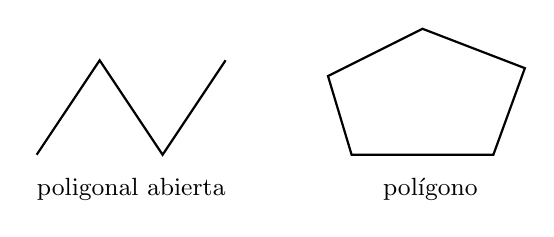
\begin{tikzpicture}[thick, every node/.append style={text height=1.6ex, text depth=0.3ex, font=\small}]
  \draw (0,0) -- (0.8,1.2) -- (1.6,0) -- (2.4,1.2);  \node[below] at (1.2,-0.15) {poligonal abierta};
  \draw (4,0) -- (5.8,0) -- (6.2,1.1) -- (4.9,1.6) -- (3.7,1) -- cycle;
                                                       \node[below] at (5,-0.15) {polígono};
\end{tikzpicture}
\end{center}

Las partes de un polígono son sus \textbf{lados} (los segmentos), sus
\textbf{vértices} (donde se unen dos lados) y sus \textbf{ángulos} (la
abertura entre dos lados, en cada vértice). Todo polígono tiene tantos lados
como vértices y como ángulos. Su nombre depende del número de lados:

\begin{center}
{\renewcommand{\arraystretch}{1.4}
\begin{tabular}{|c|c|c|c|c|}
  \hline
  3 lados & 4 lados & 5 lados & 6 lados & 8 lados\\\hline
  triángulo & cuadrilátero & pentágono & hexágono & octágono\\\hline
\end{tabular}}
\end{center}

\begin{ejemplo}[El nombre no depende del tamaño]
Un pentágono puede ser grande o pequeño, con lados iguales o distintos: si
tiene 5 lados, es un pentágono. Lo que cuenta es el número de lados.
\end{ejemplo}

\begin{aplicacion}[Señales de tránsito]
En Colombia, la señal de PARE tiene forma de octágono~\cite{mintransporte},
y la de CEDA EL PASO, de triángulo. Los conductores las reconocen por su
forma aunque estén lejos o la señal esté sucia y no se pueda leer.
\end{aplicacion}

\begin{preguntas}
\Needspace{12\baselineskip}
% Ejercicio: poligonos-4-001
\pregunta ¿Cuáles de estas cuatro figuras son polígonos? Para las que no lo
son, explica por qué.
\begin{center}
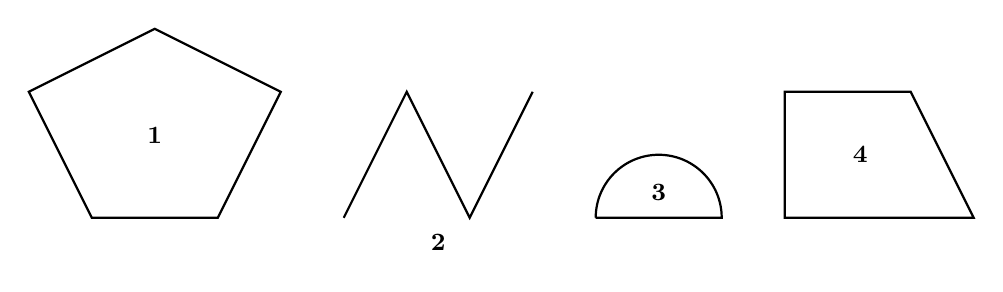
\begin{tikzpicture}[thick, scale=0.8]
  \draw (0,0) -- (2,0) -- (3,2) -- (1,3) -- (-1,2) -- cycle;  \node[etq] at (1,1.3) {1};
  \draw (4,0) -- (5,2) -- (6,0) -- (7,2);                      \node[etq] at (5.5,-0.4) {2};
  \draw (8,0) -- (10,0) arc (0:180:1);                         \node[etq] at (9,0.4) {3};
  \draw (11,0) -- (14,0) -- (13,2) -- (11,2) -- cycle;         \node[etq] at (12.2,1) {4};
\end{tikzpicture}
\end{center}
\renglones{3}

\Needspace{16\baselineskip}
% Ejercicio: poligonos-4-002
\pregunta Para cada polígono, cuenta sus lados, sus vértices y sus ángulos,
y escribe su nombre.
\begin{center}
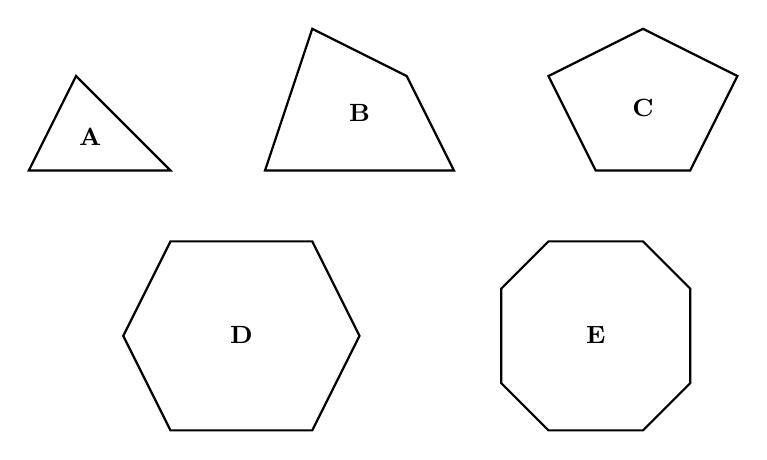
\begin{tikzpicture}[thick, scale=0.6]
  \draw (0,0) -- (3,0) -- (1,2) -- cycle;                               \node[etq] at (1.3,0.7) {A};
  \begin{scope}[xshift=5cm]
    \draw (0,0) -- (4,0) -- (3,2) -- (1,3) -- cycle;                   \node[etq] at (2,1.2) {B};
  \end{scope}
  \begin{scope}[xshift=12cm]
    \draw (0,0) -- (2,0) -- (3,2) -- (1,3) -- (-1,2) -- cycle;        \node[etq] at (1,1.3) {C};
  \end{scope}
  \begin{scope}[xshift=3cm, yshift=-5.5cm]
    \draw (0,0) -- (3,0) -- (4,2) -- (3,4) -- (0,4) -- (-1,2) -- cycle; \node[etq] at (1.5,2) {D};
  \end{scope}
  \begin{scope}[xshift=10cm, yshift=-5.5cm]
    \draw (1,0) -- (3,0) -- (4,1) -- (4,3) -- (3,4) -- (1,4) -- (0,3) -- (0,1) -- cycle;
                                                                       \node[etq] at (2,2) {E};
  \end{scope}
\end{tikzpicture}
\end{center}
{\renewcommand{\arraystretch}{1.6}
\begin{center}
\begin{tabular}{|c|c|c|c|c|}
  \hline
  \textbf{Polígono} & \textbf{Lados} & \textbf{Vértices} & \textbf{Ángulos} & \textbf{Nombre}\\\hline
  A & \hspace{1.5cm} & \hspace{1.5cm} & \hspace{1.5cm} & \hspace{3cm}\\\hline
  B & & & & \\\hline
  C & & & & \\\hline
  D & & & & \\\hline
  E & & & & \\\hline
\end{tabular}
\end{center}}
\end{preguntas}

\begin{resumen}
\begin{itemize}
  \item Un polígono es una figura plana cerrada con todos sus lados rectos.
  \item Tiene tantos lados como vértices y como ángulos.
  \item Su nombre depende del número de lados: triángulo (3), cuadrilátero (4),
        pentágono (5), hexágono (6), octágono (8).
\end{itemize}
\end{resumen}

% ---------------------------------------------------------------------
\tema{Cuadriláteros}\label{tema:cuadrilateros}

\begin{hilo}
En Hong Kong y en Yokohama, Passepartout pasea por calles con baldosas,
ventanas y cometas de papel. Todas son cuadriláteros, pero no se parecen:
unas tienen esquinas rectas, otras están «inclinadas». ¿Cómo distinguirlas?
\end{hilo}

\Needspace{9\baselineskip}
Los \textbf{cuadriláteros} son los polígonos de 4 lados. Para distinguirlos
miramos tres cosas: si sus lados miden lo mismo, si tienen lados paralelos y
si sus ángulos son rectos. Para revisarlo usamos la regla y la escuadra.

\begin{center}
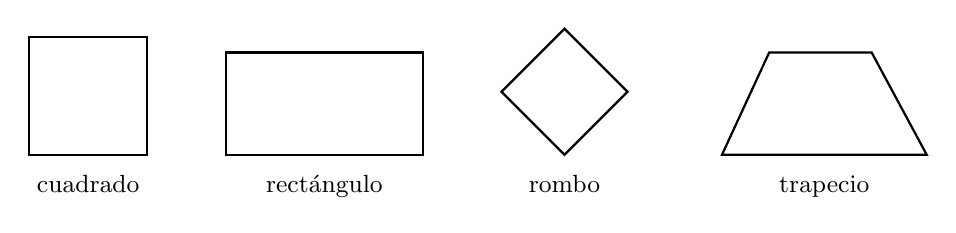
\begin{tikzpicture}[thick, every node/.append style={text height=1.6ex, text depth=0.3ex, font=\small}]
  \draw (0,0) rectangle (1.5,1.5);                    \node[below] at (0.75,-0.1) {cuadrado};
  \draw (2.5,0) rectangle (5,1.3);                    \node[below] at (3.75,-0.1) {rectángulo};
  \draw (6.8,0) -- (7.6,0.8) -- (6.8,1.6) -- (6,0.8) -- cycle; \node[below] at (6.8,-0.1) {rombo};
  \draw (8.8,0) -- (11.4,0) -- (10.7,1.3) -- (9.4,1.3) -- cycle; \node[below] at (10.1,-0.1) {trapecio};
\end{tikzpicture}
\end{center}

\begin{center}
{\renewcommand{\arraystretch}{1.4}
\begin{tabular}{|l|c|c|c|}
  \hline
  & \textbf{4 lados iguales} & \textbf{4 ángulos rectos} & \textbf{Parejas de lados paralelos}\\\hline
  Cuadrado   & sí & sí & 2\\\hline
  Rectángulo & no & sí & 2\\\hline
  Rombo      & sí & no & 2\\\hline
  Trapecio   & no & no & 1\\\hline
\end{tabular}}
\end{center}

\begin{ejemplo}[Un cuadrado es un rectángulo especial]
El rectángulo es el cuadrilátero que tiene 4 ángulos rectos. El cuadrado
también los tiene, así que el cuadrado es un rectángulo… ¡con los cuatro
lados iguales! Por la misma razón, el cuadrado también es un rombo.
\end{ejemplo}

\begin{aplicacion}[Baldosas y ventanas]
Las baldosas del piso suelen ser cuadrados o rectángulos: sus ángulos rectos
hacen que encajen unas con otras sin dejar huecos. Por eso, al construir, se
revisa con una escuadra que las esquinas de puertas y ventanas sean rectas.
\end{aplicacion}

\begin{preguntas}
\Needspace{12\baselineskip}
% Ejercicio: cuadrilateros-4-001
\pregunta Estos cinco cuadriláteros están en una cuadrícula. Con la regla y
la escuadra, revisa sus lados y sus ángulos y escribe el nombre de cada uno:
cuadrado, rectángulo, rombo, trapecio o ninguno de ellos.
\begin{center}
\begin{tikzpicture}[scale=0.42]
  \begin{scope}
    \draw[mmcLinea] (-0.5,-0.5) grid (3.5,6.5);
    \draw[very thick] (0,0) -- (3,0) -- (3,3) -- (0,3) -- cycle;  \node[etq] at (1.5,4.5) {A};
  \end{scope}
  \begin{scope}[xshift=4.5cm]
    \draw[mmcLinea] (-0.5,-0.5) grid (5.5,6.5);
    \draw[very thick] (0,0) -- (5,0) -- (5,2) -- (0,2) -- cycle;  \node[etq] at (2.5,4.5) {B};
  \end{scope}
  \begin{scope}[xshift=11cm]
    \draw[mmcLinea] (-0.5,-0.5) grid (4.5,6.5);
    \draw[very thick] (2,0) -- (4,3) -- (2,6) -- (0,3) -- cycle;  \node[etq] at (3.6,5.6) {C};
  \end{scope}
  \begin{scope}[xshift=16.5cm]
    \draw[mmcLinea] (-0.5,-0.5) grid (6.5,6.5);
    \draw[very thick] (0,0) -- (6,0) -- (4,3) -- (1,3) -- cycle;  \node[etq] at (3,4.5) {D};
  \end{scope}
  \begin{scope}[xshift=24cm]
    \draw[mmcLinea] (-0.5,-0.5) grid (5.5,6.5);
    \draw[very thick] (0,0) -- (4,0) -- (5,3) -- (1,4) -- cycle;  \node[etq] at (2.5,5.5) {E};
  \end{scope}
\end{tikzpicture}
\end{center}
A: \rule{2.2cm}{0.4pt} \; B: \rule{2.2cm}{0.4pt} \; C: \rule{2.2cm}{0.4pt} \;
D: \rule{2.2cm}{0.4pt} \; E: \rule{2.2cm}{0.4pt}

% Ejercicio: cuadrilateros-4-003
\pregunta Responde y explica:
\begin{opciones*}(2)
  \item ¿Un cuadrado es también un rectángulo?
  \item ¿Todo rombo es un cuadrado?
\end{opciones*}
\renglones{3}
\end{preguntas}

\begin{resumen}
\begin{itemize}
  \item Los cuadriláteros son polígonos de 4 lados.
  \item Se distinguen por sus lados iguales, sus lados paralelos y sus ángulos rectos.
  \item El cuadrado es a la vez rectángulo y rombo; no todo rombo es cuadrado.
\end{itemize}
\end{resumen}

% ---------------------------------------------------------------------
\tema{Figuras con polígonos}\label{tema:tangram}

\begin{hilo}
El barco de Yokohama a San Francisco tarda 22 días: el tramo más largo del
viaje. En nuestra versión de la historia, Passepartout se entretiene con un
rompecabezas chino de siete piezas. Con ellas arma un barco, un tren, una
casa\ldots\ ¡y siempre usa las mismas siete piezas!
\end{hilo}

\Needspace{9\baselineskip}
El \textbf{tangram} es un cuadrado cortado en siete polígonos: cinco
triángulos (dos grandes, uno mediano y dos pequeños), un cuadrado y un
paralelogramo (un cuadrilátero con dos parejas de lados paralelos). Con las
siete piezas, sin encimarlas, se pueden armar cientos de figuras.

\begin{center}
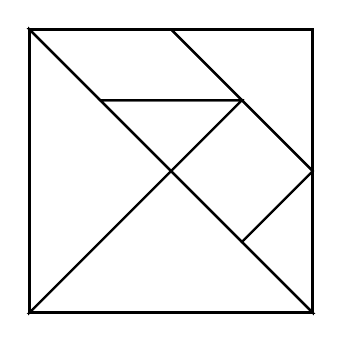
\begin{tikzpicture}[thick, scale=0.9]
  \draw (0,0) -- (4,0) -- (2,2) -- cycle;
  \draw (0,0) -- (2,2) -- (0,4) -- cycle;
  \draw (4,2) -- (4,4) -- (2,4) -- cycle;
  \draw (4,0) -- (4,2) -- (3,1) -- cycle;
  \draw (2,2) -- (3,3) -- (1,3) -- cycle;
  \draw (2,2) -- (3,1) -- (4,2) -- (3,3) -- cycle;
  \draw (0,4) -- (1,3) -- (3,3) -- (2,4) -- cycle;
  \draw[very thick] (0,0) rectangle (4,4);
\end{tikzpicture}
\end{center}

\Needspace{7\baselineskip}
\begin{ejemplo}[Armar y desarmar]
Si juntas los dos triángulos pequeños por su lado más largo, obtienes el
cuadrado del tangram. Si pones un triángulo pequeño dentro del cuadrado,
ocupa justo la mitad. Armar y desarmar figuras nos ayuda a ver cómo se
relacionan unas con otras.
\end{ejemplo}

\begin{aplicacion}[Mosaicos]
Los pisos de baldosas y los mosaicos de las paredes se hacen juntando
polígonos que encajan sin dejar huecos, como las piezas del tangram. Muchos
artistas crean figuras de animales y personas solo con triángulos y
cuadriláteros.
\end{aplicacion}

\begin{preguntas}
% Ejercicio: tangram-4-001
\pregunta Observa las siete piezas del tangram. ¿Cuántas son triángulos?
¿Cuáles son cuadriláteros y cómo se llaman?
\renglones{2}

% Ejercicio: tangram-4-003
\pregunta Con los dos triángulos pequeños del tangram se pueden armar tres
figuras distintas juntando dos lados iguales. Dibújalas y escribe su nombre.
\espacio{4cm}
\end{preguntas}

\begin{resumen}
\begin{itemize}
  \item El tangram tiene 7 piezas: 5 triángulos, 1 cuadrado y 1 paralelogramo.
  \item Juntando polígonos se forman otros polígonos: dos triángulos pueden
        formar un cuadrado, un triángulo más grande o un paralelogramo.
\end{itemize}
\end{resumen}

% ---------------------------------------------------------------------
% 5. Cierre del hilo conductor
% ---------------------------------------------------------------------
\seccion{Cierre: el día que apareció}

Fogg llega a Londres convencido de que perdió la apuesta por un día. Pero se
equivocaba: como viajó siempre hacia el este, hacia donde sale el Sol, cada
día le duró unos minutos menos. Verne hace la cuenta: la vuelta a la Tierra
tiene 360 grados, y por cada grado se ganan 4 minutos; $360 \times 4$ minutos
son 24 horas, ¡un día completo!~\cite{verne} Fogg llega a tiempo y gana.

Como Fogg, este trimestre recorrimos un camino por etapas: de las líneas a
los polígonos, de los polígonos a los cuadriláteros y de ahí a las figuras
armadas. En el próximo trimestre aprenderemos a \textbf{medir}: longitudes,
contornos y superficies.

% ---------------------------------------------------------------------
% 6. Evaluación (secciones institucionales)
% ---------------------------------------------------------------------
\matrizevaluacion
  {Reconoce rectas paralelas, perpendiculares y secantes, polígonos y cuadriláteros por sus propiedades.}
  {Traza paralelas y perpendiculares con regla y escuadra, clasifica cuadriláteros y arma figuras con polígonos.}
  {Planea y revisa su trabajo con cuidado, paso por paso.}
  {Comparte materiales e ideas en el trabajo en grupo y respeta las creaciones de los demás.}

\autoevaluacion

\seguimientodocente

% ---------------------------------------------------------------------
% 7. Referencias
% ---------------------------------------------------------------------
\begin{referencias}
% verificado: https://theconversation.com/the-history-and-mystery-of-tangram-the-childrens-puzzle-game-that-harbours-a-mathematical-paradox-or-two-190529 — T. Britz, 28 dic. 2022: invento chino hacia 1800, 7 piezas, fiebre en Europa 1817–18
\bibitem{britz} Britz, T. (2022, 28 de diciembre). The history and mystery of Tangram,
  the children's puzzle game that harbours a mathematical paradox or two. \emph{The Conversation}.
% verificado: https://jules-verne.net/l-oeuvre/les-voyages-extraordinaires/1872-1873-1-le-tour-du-monde-en-quatre-vingts-jours/ — Le Temps, nov.–dic. 1872; Hetzel, 30 ene. 1873
\bibitem{cijv} Centre international Jules Verne (s.\,f.). \emph{Le Tour du monde en
  quatre-vingts jours} (1872--1873). Amiens.
% verificado: https://mathcs.clarku.edu/~djoyce/elements/bookI/bookI.html — Libro I, definición 23 (rectas paralelas)
\bibitem{euclides} Euclides (ca. 300 a.\,C.). \emph{Elementos}, Libro I (ed. electrónica
  de D. E. Joyce). Clark University.
% verificado: https://gblumen.mineducacion.gov.co/cgi-bin/koha/opac-detail.pl?biblionumber=4785 — MEN 2016
\bibitem{mendba} Ministerio de Educación Nacional (2016). \emph{Derechos
  Básicos de Aprendizaje V.2: Matemáticas}. Bogotá: MEN.
% verificado: https://operaciones.colombiacompra.gov.co/sites/cce_public/files/documentos_adicionales_oc/ficha_tecnica_48.pdf — ficha técnica oficial que cita la Resolución 1885 de 2015: «misma forma … de la señal SR-01 Pare … un octágono»
\bibitem{mintransporte} Ministerio de Transporte (2015). \emph{Manual de señalización
  vial} (Resolución 1885 de 2015). Bogotá: Ministerio de Transporte.
% verificado: https://www.womenshistory.org/education-resources/biographies/nellie-bly-0 — viaje de 72 días (1889), New York World, inspirado en Verne
\bibitem{nwhm} National Women's History Museum (s.\,f.). \emph{Nellie Bly}.
% verificado: https://fr.wikisource.org/wiki/Le_Tour_du_monde_en_quatre-vingts_jours/Chapitre_3 — cap. III (frase, apuesta, itinerario de 80 días); cap. XXXVII (360 × 4 min = 24 h): https://fr.wikisource.org/wiki/Le_Tour_du_monde_en_quatre-vingts_jours/Chapitre_37
\bibitem{verne} Verne, J. (1873). \emph{Le Tour du monde en quatre-vingts jours}.
  París: Hetzel.
\end{referencias}

\end{document}
